\section*{Systemanalyse L�sungen}\label{MA2-systemanalyse-loesungen}

\ifintegriereaufgaben Regeln und Beispiele, die zur Bearbeitung der Aufgaben hilfreich sind, finden Sie im Skript\wennreferenzvorhanden{MA2-systemanalyse}{ (Abschnitt \abschnittsverweis{MA2-systemanalyse})}.\fi


\begin{exercisebox}[Polstellen (�bertragungsfunktion Laplace) ] % s=-1, s=-2
Gegeben sei

\[
	H(s)=\frac{2}{s^2+3s+2} = \frac{2}{(s+1)\cdot (s+2)}
\]


\begin{enumerate}

	\item Die Faktorisierung des Nennerpolynoms liefert die Polstellen \(s=-1\) und \(s=-2\)\,.
		\[ s_{1,2} = \dfrac{(-3) \pm \sqrt{ 3^2 - 4\cdot  2 }}{2} = \dfrac{-3 \pm 1}{2}  \Rightarrow \, H(s)=\frac{2}{s^2+3s+2} = \frac{2}{(s+1)\cdot (s+2)} \]

\item Skizzieren Sie die Lage der Polstellen in der komplexen Ebene:

\begin{center}
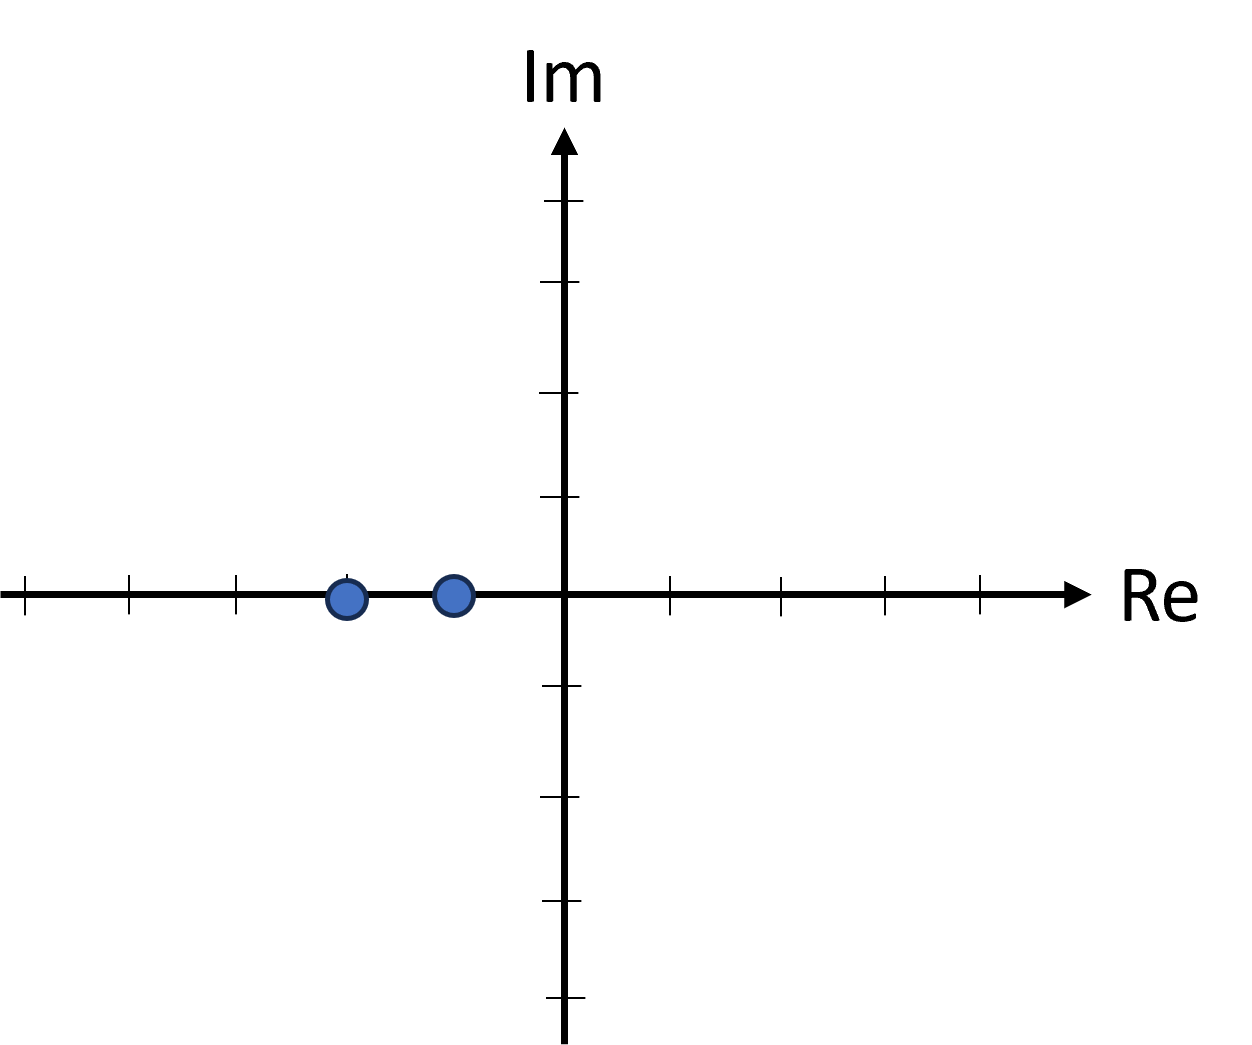
\includegraphics[width=5cm]{../Mathematik_2/Bilder/systemanalyse_reelle_polstellen.png}
\end{center}

\end{enumerate}


\end{exercisebox}

\begin{exercisebox}[Polstellen (�bertragungsfunktion Laplace)] % s = -1 pm 2i
Gegeben sei

\[
H(s)=\frac{1}{s^2+2s+5}.
\]

\begin{enumerate}

	\item Bestimmen Sie die Polstellen: das Nennerpolynom ist ein quadratischer Term. Die Nullstellen und damit die Polstellen von \(H\) sind komplex:
	\[ s_{1,2} = \dfrac{(-2) \pm \sqrt{ \textcolor{red}{|} 2^2 - 4\cdot  5\textcolor{red}{|} } \,\textcolor{red}{i} }{2 } = -1 \pm 2\, i  \Rightarrow \, H(s)=\frac{2}{s^2+2s+5} = \frac{2}{(s+1+2i)\cdot (s+1-2i)} \]

\item Skizzieren Sie die Lage der Polstellen in der komplexen Ebene.
\begin{center}
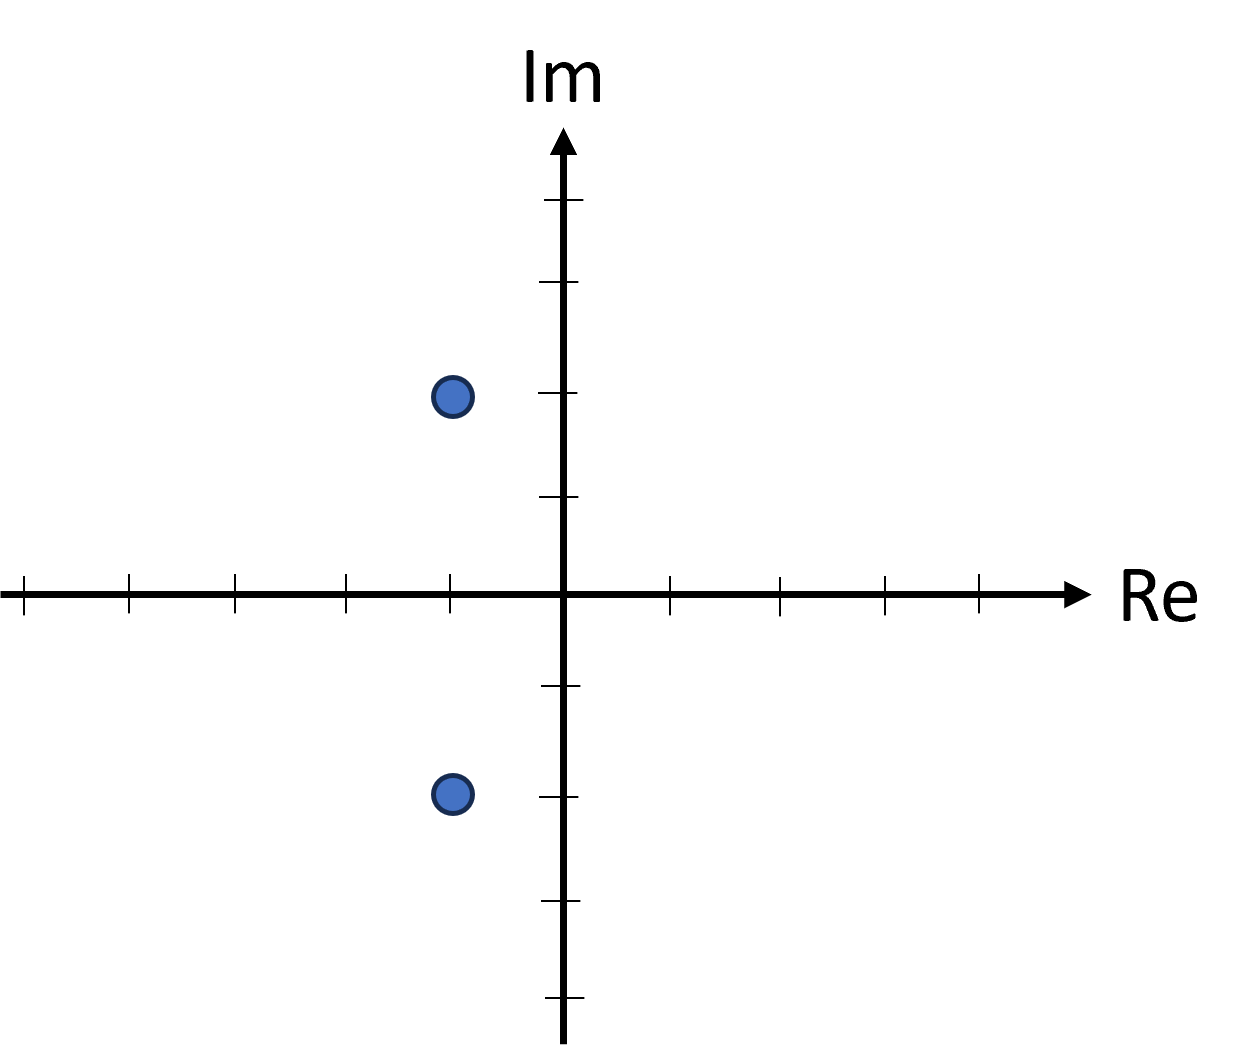
\includegraphics[width=5cm]{../Mathematik_2/Bilder/systemanalyse_konjugiert_komplexe_polstellen.png}
\end{center}

\item Was bedeutet das f�r das Zeitverhalten eines Systems? Das System ist asymptotisch stabil, weil die pyhsikalische L�sung f�r \(t\to \infty\) verschwindet.

\end{enumerate}

\end{exercisebox}

\begin{exercisebox}[Polstellen (�bertragungsfunktion Laplace)] % s = -1 pm 2i
Die folgende Skizze zeigt die Polstellen einer �bertragungsfunktion in der komplexen Ebene.

\begin{center}
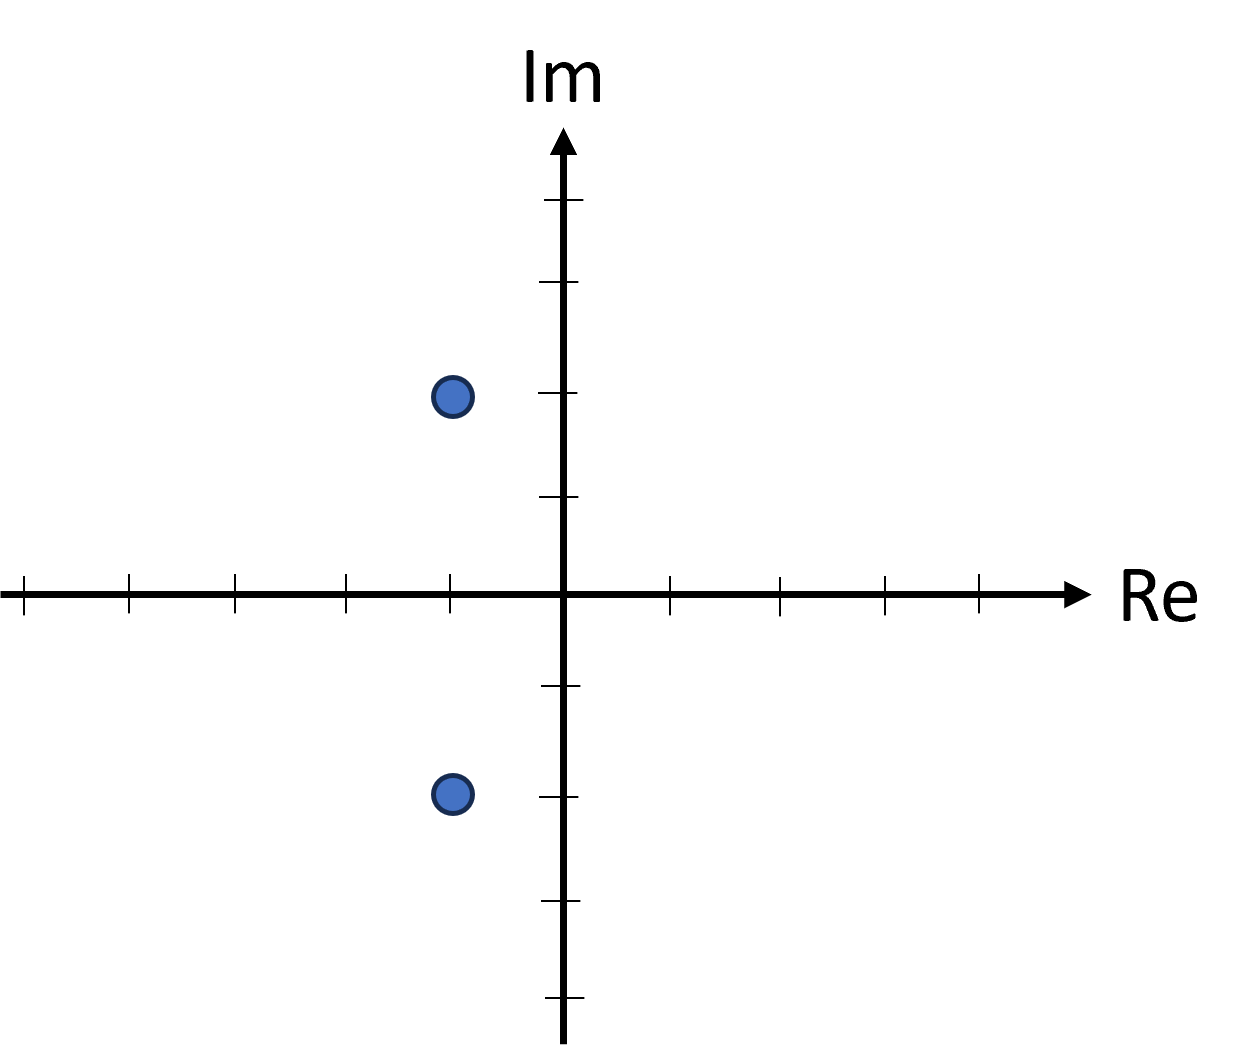
\includegraphics[width=5cm]{../Mathematik_2/Bilder/systemanalyse_konjugiert_komplexe_polstellen.png}
\end{center}

\begin{enumerate}
	\item Lesen Sie die Polstellen aus der Skizze ab. \(s_{1,2} = -1 \pm 2i\)
\item Geben Sie ein m�gliches Polynom an, das im Nenner der �bertragungsfunktion stehen k�nnte: \(p(s) = (s+1+ 2i)\cdot (s+1-2i)\).
\end{enumerate}

\end{exercisebox}

